%%%%%%%%%%%%%%%%%%%%%%%%%%%%%%%%%%%%%%%%%%%%%%%%%%%%%%%%%%%%%%%%%%%%%%%%%%%%%%%
%
% SIINTEC Template Example Document
% Simpósio Internacional de Inovação e Tecnologia
% International Symposium on Innovative Technologies
%
% Author: Nelson Alves Ferreira Neto
% Email: nelsonafn@gmail.com
% Date: July 29, 2025
% Version: 1.0
%
% Description: Example document demonstrating the use of the SIINTEC LaTeX class
%              for symposium papers. This template illustrates the correct
%              formatting of academic articles according to the event guidelines.
%
% Features demonstrated:
%   - Title, author, and affiliation formatting with custom commands
%   - Abstract with keywords and abbreviations in single column
%   - Section hierarchy and automatic numbering
%   - Tables and figures with captions and cross-references
%   - Numbered mathematical equations
%   - Vancouver reference style with square brackets
%   - Two-column layout for main content
%   - Custom header with logo and ISSN
%
% Usage instructions:
%   1. Replace the example content with your article
%   2. Update title, authors, and affiliations using \siintectitle, \siintecauthor, \siintecaffil
%   3. Fill in the abstract, keywords, and abbreviations in \siintecabstract
%   4. Insert your sections, figures, tables, and references
%   5. Compile with pdflatex and bibtex (if using automatic references)
%
% Requirements:
%   - siintec.cls (event class)
%   - siintec.png (event logo)
%   - Images used in figures
%   - Reference file refs.bib
%
% 2025 Conference Theme:
%   "Quantum Technologies: The information revolution that will change the future"
%
%%%%%%%%%%%%%%%%%%%%%%%%%%%%%%%%%%%%%%%%%%%%%%%%%%%%%%%%%%%%%%%%%%%%%%%%%%%%%%%

% Loads the SIINTEC class (based on article, with custom formatting)
\documentclass{siintec}

%--------------------------- ARTICLE METADATA -------------------------------%

% Article title (max. 3 lines, Times 12pt bold, centered)
\siintectitle{Template for Preparing an Article}

% Authors and affiliations (use [*] for corresponding author, [n] for multiple affiliations)
\siintecauthor[*,1]{Author One}
\siintecauthor[2]{Author Two}
\siintecauthor[3]{Author Three}
\siintecaffil[1]{Organization Name, Department Name, City, State, Country}
\siintecaffil[2]{Organization Name, Department Name, City, State, Country}
\siintecaffil[3]{Organization Name, Department Name, City, State, Country}
\siintecaffil[*]{Corresponding author: institution; addresses; author3@email}

% Remove the default LaTeX date
\siintecdate

%--------------------------- BEGIN DOCUMENT ---------------------------------%

\begin{document}

%--------------------------- FRONT MATTER -----------------------------------%

% Formatted abstract (single column, then two columns)
% Parameters: {abstract text}{keywords}{abbreviations}
\siintecabstract{This document gives formatting instructions for authors preparing papers for publication in the SIINTEC. Authors are encouraged to prepare manuscripts directly using this template. Use Times New Roman, 10 (Font Size), Bold (or Bold Italic for name of species \textit{Candida albicans}), and >1800 to 2000 characters with spaces.}{Times New Roman, 10 (Font Size), Bold (or Bold Italic for name of species \textit{Candida albicans}). Use the minimum of 3 words and the maximum of 5 words separated by a dot.}{Times New Roman, 10 (Font Size), Bold. Abbreviation + comma + the meaning of the abbreviation. They should be separated by a dot.}

%--------------------------- MAIN CONTENT -----------------------------------%

% Main section (bold, 12pt, automatic numbering)
\section{Introdução to Font Sizes for Papers}
% Main text: Times 12pt, 1.5 spacing, justified, two columns
{\siintecmainfont
To use this template, you will need to (1) apply the embedded styles to each paragraph-level item in your manuscript or (2) use the specifications shown in Table 1 to format your manuscript, with this template as a visual guide. The page limit for the article is between 6 (six) and 8 (eight) pages, considering text, tables, figures and photos.
}

% Example of table with SIINTEC formatting using custom font command
\begin{table}[ht]
\centering
\caption{\siinteccaptionfont Font sizes and styles for SIINTEC.} % Caption above the table
\label{tab:font-sizes}
\renewcommand{\arraystretch}{1.5}
{\siintectablefont
\setlength{\tabcolsep}{1pt}
\begin{tabular}{|c|c|c|c|c|}
\hline
\textbf{Font Size} & \multicolumn{4}{c|}{\textbf{Appearance (in Time New Roman)}} \\
\cline{2-5}
 & \textbf{Regular} & \textbf{Bold} & \textbf{Italic} & \textbf{Underline} \\
\hline
10 &
\begin{tabular}[c]{@{}l@{}}Author affil.\\ Abrv. of tab.,\\ figures, box;\\ References\end{tabular} &
\begin{tabular}[c]{@{}l@{}}Abst. body\\ Keywords,\\ Abbrev. \end{tabular} &
\begin{tabular}[c]{@{}l@{}}Corresp. auth\\ Receiv Line\end{tabular} &
\\
\hline
12 &
\begin{tabular}[c]{@{}l@{}}Main text,\\ Desc. of fig.,\\ tab. box \\ and graphics\\ Sec. head -- l2\end{tabular} &
\begin{tabular}[c]{@{}l@{}}Sec. headl. \\-- level 1\end{tabular} &
\begin{tabular}[c]{@{}l@{}}Sec. headl. \\-- level 3\end{tabular} &
\begin{tabular}[c]{@{}l@{}}Sec. headl. \\-- level 2\end{tabular} \\
\hline
\end{tabular}
}
\end{table}

% New section (example of template usage)
\section{Ease of Use}
An easy way to comply with the paper formatting requirements is to use this document as a template and simply type your text into it.

The template is used to format your paper and style the text. All margins, column widths, line spaces, and text fonts are prescribed; please do not alter them.

% Subsection: page layout
\subsection{Page Layout}
Your paper must use a page size corresponding to A4 which is 210 mm wide and 297 mm long. The margins are set as follows: top= 15 mm, bottom= 15 mm, right=17.5 mm, left = 20 mm. Your paper must be in two column format with a space of 1.93 characters between columns.

% Subsubsections: detailed formatting instructions
\subsubsection{Front Matter}
The title should in Times New Roman, font size 12, bold. Do not use more than 3 lines. The title must be separated from the authors by a double paragraph space (in 12-point font). Use numerical superscript callouts as shown in this template to link authors with their affiliations.
Corresponding author should be denoted with an asterisk as shown. E-mail address is compulsory for the corresponding author.
The authors must be separated from the affiliations by a single paragraph space (in 12-point font).

\subsubsection{Text Font}
The main text should be in Times New Roman font size 12, double space. Paper title must be centered, bold, regular font size 12. Author names must be centered, bold, regular font size 10. Author affiliation must be regular font size 10, italic. Email address must be centered, italic, font size 10. Recommended font sizes are shown in Table 1. No more than 3 levels of headings should be used. Level 1 heading must be left-justified, bold, regular font size 12. Level 2 headings must be left-justified, regular, underline, regular font size 12 and numbered. Level 3 heading must be left-justified, italic font size 10, and the first letter of each word capitalized.

\subsubsection{Equations}
Display equations should be broken and aligned for two-column display unless spanning across two columns is essential. Equations should be centered with equation numbers set flush right. If using MathType, use the Format Equations feature to format all equations as Times + Symbol  or Calibri Math10.

\begin{equation}
x = \frac{-b \pm \sqrt{b^2 - 4ac}}{2a}
\end{equation}

\subsubsection{Tables}
Styles for table title, table head, and table text are provided. Tables could be in one or two columns, and be placed near their first mention in the body. Tables, figures and graphics need to be placed on separate pages at the back of the manuscript.

\subsubsection{Figures}
As with tables and equations, figures could be set in one or two columns. The resolution of image should be adequate to reveal the important detail in the figure (300 dpi).

\subsubsection{Figure Captions}
Figure descriptions should be placed above the figures (however, abbreviations, explanations, or figure legends should be placed below the figure). Figures must be numbered using Arabic numerals, in 12 pt bold font, and the description should be in regular (non-bold) font. The legends below the Figure should be in 10 pt regular font, and single space. Single-line captions (e.g., \autoref{fig:biochip}) should be left-aligned, while multi-line captions should be justified (e.g., \autoref{fig:edfa-setup}). Captions with figure numbers must be placed after their respective figures, as shown in \autoref{fig:edfa-setup}.

% Example of figure with caption and explanatory legends
\begin{figure}[ht]
    \centering
    \caption{Forward single pass experimental set-up for evaluating EDFA performance.}
    \label{fig:edfa-setup}
        \vspace{0.5em}
    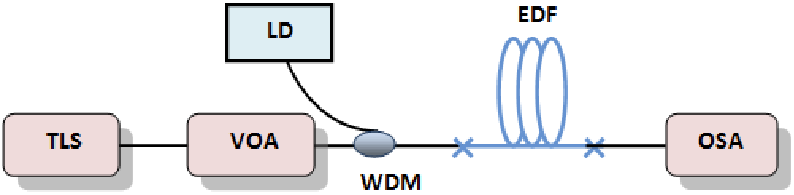
\includegraphics[width=0.7\linewidth]{edfa-setup.png}
    \begin{flushleft}
    \siintecbibliographyfont
    LD, lase diode. OSA, optical spectrum analyzer. TLS, tunable laser source. VOA, variable optical attenuator. Abbreviations or legends should be separated by a dot.
    \end{flushleft}
\end{figure}

% Example of simple figure
\begin{figure}[ht]
    \centering
    \caption{Biochip Reader integrated circuit.}
    \label{fig:biochip}
        \vspace{0.5em}
    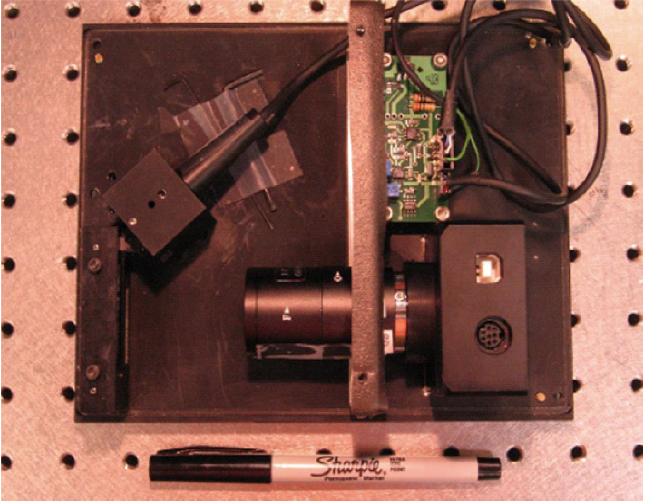
\includegraphics[width=0.7\linewidth]{biochip.png}
\end{figure}

% Example of graphic with TikZ
\begin{graphic}[ht]
    \centering
    \caption{Diagram example created with TikZ.}
    \label{grph:tikz}
    \begin{tikzpicture}[scale=1.2]
      % Axes
      \draw[thick,->] (0,0) -- (4,0) node[anchor=west] {};
      \draw[thick,->] (0,0) -- (0,3) node[anchor=south] {};
      % X axis label (bold)
      \node[anchor=west, font=\bfseries] at (-0.5,3.2) {X axis};
      % Mathematical curve
      \draw[thick,domain=0:3.5,smooth,samples=50] plot(\x,{2*sin(60*\x)*exp(-0.3*\x)+1+0.3*\x});
      % Arrow on X axis
      \draw[thick] (3.95,-0.08) -- (4,0) -- (3.95,0.08);
    \end{tikzpicture}
\end{graphic}

\subsubsection{Table Captions}
Table heads should appear above the tables. Tables must be numbered using Arabic numerals. Table captions must be left-justified and in 12 pt Regular font. Captions with table numbers must be placed before their associated tables, as shown in \autoref{tab:font-sizes}.

%--------------------------- REFERENCES --------------------------------------%

\section{References Formats}
The heading of the References section must not be numbered. All reference items must be in 10 pt font. Number the reference items consecutively in square brackets (e.g. \cite{fogg2003}). When referring to a reference item, please simply use the reference number, as in (name of the first author + and colleagues (if applicable) + year of publication + number of the reference \cite{hirsh2002}.  Do not use "Ref. \cite{eckes2000}" or "Reference \cite{eckes2000}" use the name of the author(s) as described before".  Multiple references are each numbered with separate brackets (e.g. \cite{fogg2003}, \cite{hirsh2002,eckes2000}).
A complete reference should follow the Vancouver style, including the name(s) of the author(s) and/or editor(s), the title of the article, the name of the journal, book, or conference proceedings, the name of the publisher, the year of publication. This should be followed by the volume, issue number (if applicable), and page range. At the end, include the DOI (if available).
The basic principle is that the reference should be sufficiently detailed so that the reader can easily locate the source and assess its authority and objectivity.

% Vancouver style reference examples
\textbf{\underline{Vancouver Style}}

{\siintecbibliographyfont

Book\\
\textbf{Standard format:}\\
Author(s). Title of the book. Edition (if not first). Place of publication: Publisher; Year. p. pages (if applicable).\\
\textbf{Example:}\\
1. Fogg BJ. Persuasive technology: using computers to change what we think and do. Boston: Morgan Kaufmann Publishers; 2003. p. 30–5.\\

Journal Articles\\
\textbf{Standard format:}\\
Author(s). Title of article. Journal Title. Year;Volume(Issue):Pages.\\
\textbf{Example:}\\
2. Hirsh H, Coen MH, Mozer MC, Hasha R, Flanagan JL. Room service, AI-style. IEEE Intell Syst. 2002;14(2):8–19.\\

Conference Proceedings\\
\textbf{Standard format:}\\
Author(s). Title of article. In: Title of conference. Place of publication: Publisher; Year. p. pages.\\
\textbf{Example:}\\
3. Leclercq P, Heylighen A. 5.8 analogies per hour: A designer's view on analogical reasoning. In: 7th International Conference on Artificial Intelligence in Design. Dordrecht: Kluwer Academic Publishers; 2016. p. 285–303.\\

E-Books\\
\textbf{Standard format:}\\
Author(s). Title of e-book [e-book]. Place of publication: Publisher; Year [cited Year Month Day]. Available from: URL\\
\textbf{Example:}\\
4. Eckes T. The developmental social psychology of gender [e-book]. Mahwah (NJ): Lawrence Erlbaum; 2000 [cited 2025 May 27]. Available from: netLibrary e-book.\\

E-Journal Articles\\
\textbf{Standard format:}\\
Author(s). Title of article. Journal Title [Internet]. Year [cited Year Month Day];Volume(Issue):Pages. Available from: URL\\
\textbf{Example:}\\
5. Steiner A. Understanding hypertext in the context of reading on the web: Language learners' experience. Curr Issues Educ [Internet]. 2013 [cited 2025 May 27];6(12):2015–219. Available from: \url{http://cie.ed.asu.edu/v6/n12/}\\

}


%--------------------------- ACKNOWLEDGEMENTS -------------------------------%

\section*{Acknowlegement}
The heading of the Acknowledgment section and the References section must not be numbered.

%--------------------------- BIBLIOGRAPHY -----------------------------------%

% Only keep the bibliography command, style is now set by the class
\section*{References}
\bibliography{refs}

\end{document}
